%%%%%%%%%%%%%%%%%%%%%%%%%%%%%%%%%%%%%%%%%%%%%%%%%%%%%%%%%%%%
%%  This Beamer template was created by Cameron Bracken.
%%  Anyone can freely use or modify it for any purpose
%%  without attribution.
%%
%%  The current presentation created by Jeferson L. R. Souza (jefecomp) is based on the template created by Cameron Bracken. 
%%  
%%  Small modifications have been introduced and anyone is free to use such modified version.
%%
%% Last Modified: June 14, 2015.

\documentclass[xcolor=x11names,compress]{beamer}

%% General document %%%%%%%%%%%%%%%%%%%%%%%%%%%%%%%%%%
\usepackage{graphicx}
\usepackage{tikz}
\usetikzlibrary{decorations.fractals}
%%%%%%%%%%%%%%%%%%%%%%%%%%%%%%%%%%%%%%%%%%%%%%%%%%%%%%

%Hyperref
\usepackage{hyperref}

%Multirow package
\usepackage{multirow} 

%Math packages
\usepackage{amsmath}
\usepackage{textcomp}


%% Beamer Layout %%%%%%%%%%%%%%%%%%%%%%%%%%%%%%%%%%
\useoutertheme[footline=authorinstitutetitle,subsection=false,shadow]{miniframes}
\useinnertheme{default}
\usefonttheme{professionalfonts}
\usepackage{mathpazo}

\setbeamerfont{title like}{shape=\scshape,series=\bfseries}
\setbeamerfont{frametitle}{shape=\scshape,series=\bfseries}
\setbeamerfont{alerted text}{series=\bfseries}

\setbeamercolor*{lower separation line head}{bg=Green3} 
\setbeamercolor*{upper separation line foot}{bg=Green3} 
\setbeamercolor*{normal text}{fg=black,bg=white} 
\setbeamercolor*{alerted text}{fg=black,bg=black!10} 
\setbeamercolor*{example text}{fg=black} 
\setbeamercolor*{structure}{fg=black}
 
\setbeamercolor*{palette tertiary}{fg=black,bg=black!3} 
\setbeamercolor*{palette quaternary}{fg=black,bg=black!10} 

%%%%%%%%%%%%%%%%%%%%%%%%%%%%%%%%%%%%%%%%%%%%%%%%%%

\setbeamertemplate{blocks}[rounded] [shadow=true]
\setbeamertemplate{frametitle continuation}[from second][(Continuação)]

%%  declaring picture extensions and default path
\DeclareGraphicsExtensions{.png, .jpg, .pdf}
\graphicspath{{pictures/}}

%% Supporting source code lists
\usepackage{listings}
\lstset{breakatwhitespace,
language=Java,
columns=fullflexible,
keepspaces,
breaklines,
tabsize=3, 
showstringspaces=false,
extendedchars=true}

%Text position
\usepackage{textpos}
\setlength{\TPHorizModule}{128mm}
\setlength{\TPVertModule}{96mm}

\usepackage{array}

%Puting text and other float elements over pictures
\usepackage[percent]{overpic}

%% Hyperlinks over all the document
\usepackage{hyperref}

%% Controlling text alignment
\usepackage{ragged2e}

%% Framed text
\usepackage{framed}

%% Math packages
\usepackage{amsmath}

\begin{document}

\title[Levantamento de Requisitos \hskip35mm \insertframenumber / \inserttotalframenumber  \hskip32mm \inserttitlegraphic]{Levantamento de Requisitos \\[4mm]
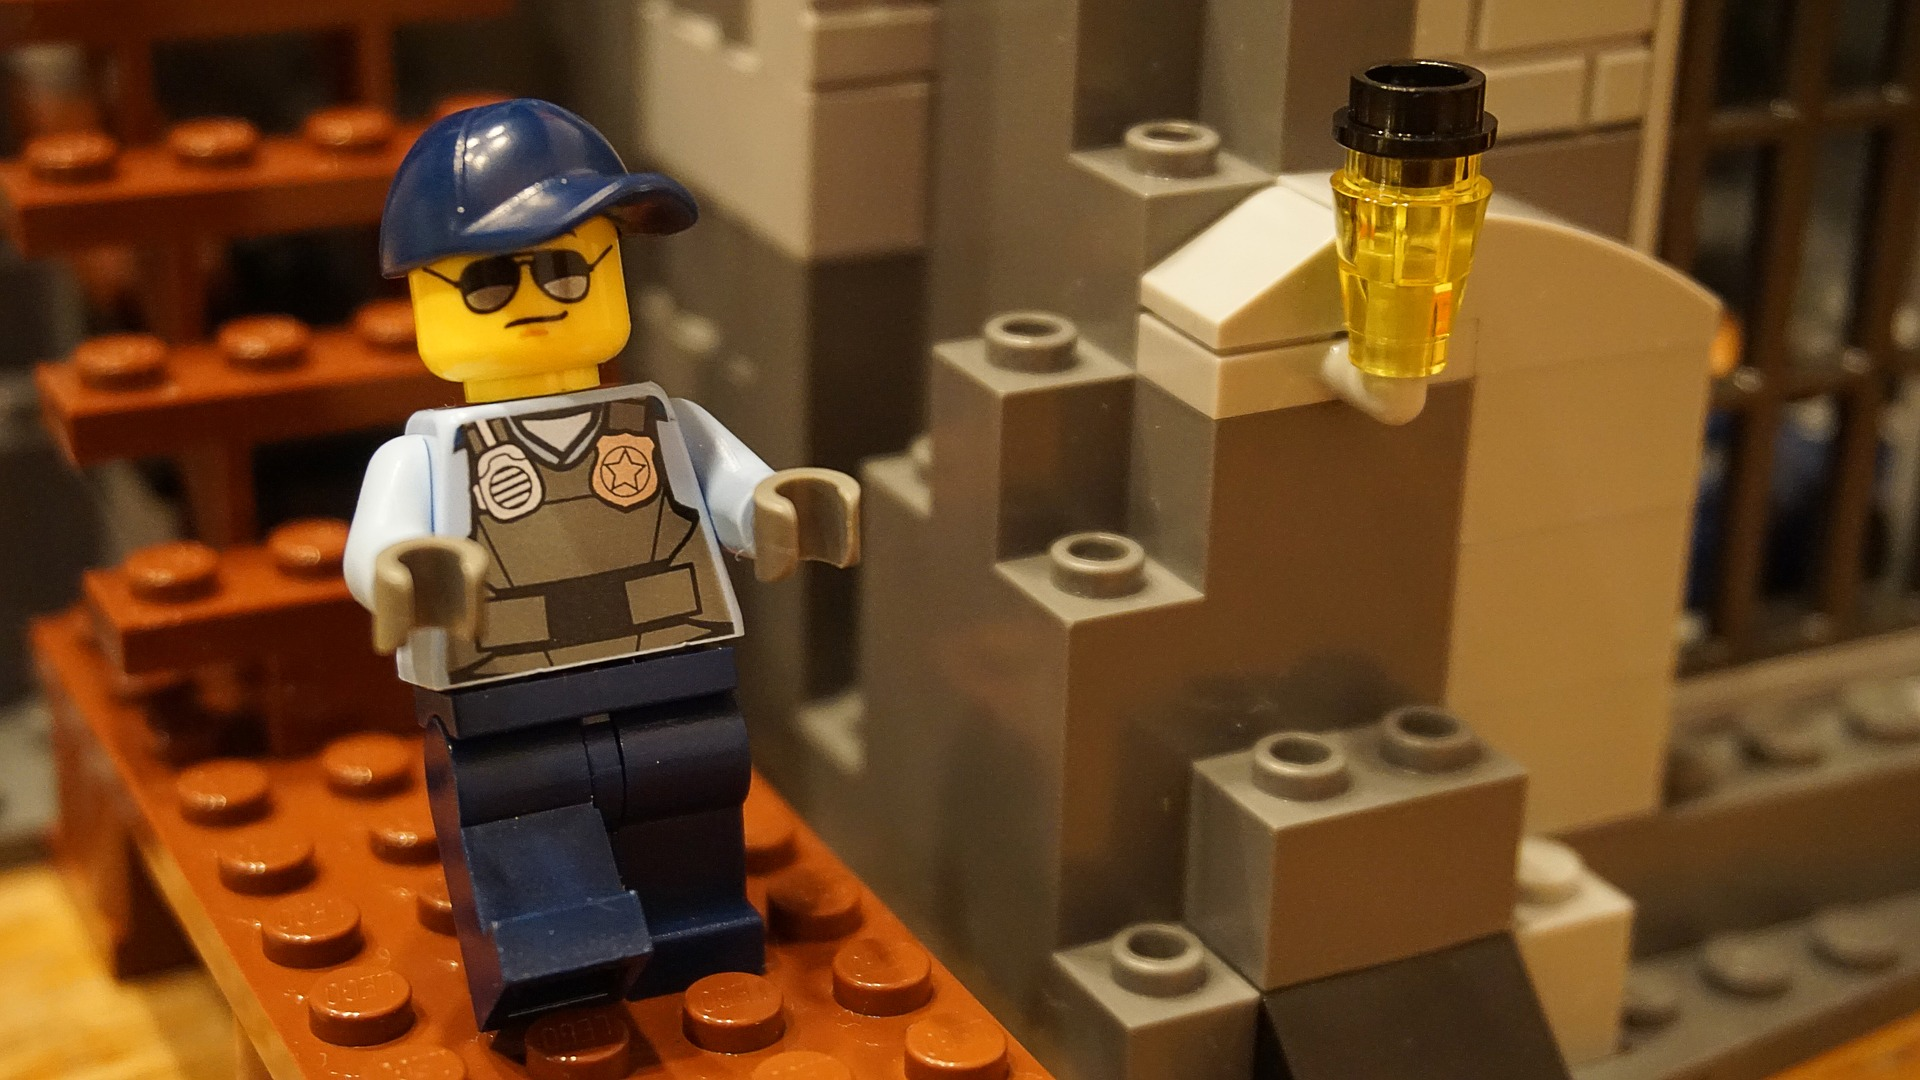
\includegraphics[keepaspectratio,width=.5\textwidth]{lego-ppr}}
\author[@2018 Prof. Jeferson Souza, MSc (jefecomp) - All rights reserved.]{
	\textcolor{blue}{Prof. Jeferson Souza, MSc.} \\[1mm] 
	\textcolor{blue}{\textit{{\footnotesize (jefecomp) }}}\\[1.5mm]
	 \underline{{\footnotesize jeferson.souza@udesc.br}}
	 \vspace*{1mm}
}
\institute[]{
\includegraphics[keepaspectratio,width=.5\textwidth]{template/logo_udesc_joinville_horizontal_assinatura}
}

\date{}

\titlegraphic{
\includegraphics[keepaspectratio,width=.2\textwidth]{template/logo_udesc_joinville_horizontal_assinatura}}

%%%%%%%%%%%%%%%%%%%%%%%%%%%%%%%%%%%%%%%%%%%%%%%%%%%%%%
%%%%%%%%%%%%%%%%%%%%%%%%%%%%%%%%%%%%%%%%%%%%%%%%%%%%%%
\begin{frame}[plain,noframenumbering]
\titlepage
\end{frame}

%%%%%%%%%%%%%%%%%%%%%%%%%%%%%%%%%%%%%%%%%%%%%%%%%%%%%%
%%%%%%%%%%%%%%%%%%%%%%%%%%%%%%%%%%%%%%%%%%%%%%%%%%%%%%
\section{Introdução}
\subsection{Introdução}
\begin{frame}{O que é um Requisito?}

\begin{alertblock}{\textbf{Requisito}}
Um requisito pode ser definido como uma necessidade, algo que é desejado e esperado. Exemplo: prestar atenção no professor é um requisito da disciplina Projeto de Programas (:-D).
\end{alertblock}

\end{frame}

\begin{frame}{Para que serve o Levantamento de Requisitos?}

\begin{alertblock}{\textbf{Finalidade}}
Descobrir e entender as reais necessidades do cliente, ou seja, o que o cliente realmente quer.
\end{alertblock}

\pause

\begin{alertblock}{\textbf{Ahh professor, isso é fácil....}}

Nãooooooooo! O levantamento de requisitos está longe de ser uma tarefa fácil...

\end{alertblock}

\pause 

\begin{alertblock}{\textbf{Por que?}}

Nem sempre o cliente sabe as suas reais necessidades, ou seja, não sabe muito bem o que quer.

\end{alertblock}

\end{frame}


\begin{frame}[allowframebreaks=.8]{O que esperar do Levantamento de Requisitos?}

\begin{itemize}
\itemsep 5mm

\item Compreender quais são as reais necessidades do cliente (o que o cliente realmente quer);

\item Compreender o negócio o qual a solução (produto/software) será desenvolvida;

\item Identificar pessoas que podem auxiliar no processo de especificação e entendimento dos requisitos;

\item Elaborar uma lista com os requisitos que descrevem as necessidades do cliente;

\item Identificar e remover ambiguidades entre os requisitos;

\item Criar casos de uso para auxiliar a identificação dos principais requisitos;

\item Em alguns casos, pode-se também produzir um protótipo simples para auxiliar a definição e o entendimento dos requisitos.
\end{itemize}

\end{frame}

%%%%%%%%%%%%%%%%%%%%%%%%%%%%%%%%%%%%%%%%%%%%%%%%%%%%%%
%%%%%%%%%%%%%%%%%%%%%%%%%%%%%%%%%%%%%%%%%%%%%%%%%%%%%%
\section{Dificuldades}
\subsection{Dificuldades}

\begin{frame}{Principais dificuldades}

\begin{itemize}
\itemsep 5mm

\item Definição de escopo;

\item Entendimento do problema/necessidade;

\item Mudanças.

\end{itemize}

\end{frame}

\begin{frame}{Definição de escopo}

\begin{alertblock}{\textbf{Problemas de escopo}}
Durante o levantamento de requisitos os limites da solução (produto/software) não ficam muito bem definidos, ou o cliente especifica detalhes técnicos que mais confundem do que ajudam a definir claramente os objetivos do sistema.
\end{alertblock}

\end{frame}

\begin{frame}{Entendimento do Problema/Necessidade}

\begin{alertblock}{\textbf{Entendimento}}
O cliente tem dificuldade para saber o que realmente quer, um baixo conhecimento do seu próprio negócio, e/ou problemas de comunicar suas necessidades. 
\end{alertblock}

\end{frame}

\begin{frame}{Mudanças}

\begin{alertblock}{\textbf{Ahhh a passagem do tempo....}}
Os requisitos podem mudar com o passar do tempo, e então atualizações precisam ser realizadas nos requisitos já definidos anteriormente.
\end{alertblock}

\end{frame}

%%%%%%%%%%%%%%%%%%%%%%%%%%%%%%%%%%%%%%%%%%%%%%%%%%%%%%
%%%%%%%%%%%%%%%%%%%%%%%%%%%%%%%%%%%%%%%%%%%%%%%%%%%%%%
\section{Início}
\subsection{Início}

\begin{frame}{Iniciar o Levantamento de Requisitos}

\begin{alertblock}{\textbf{O início}}

O método mais comum para iniciar o levantamento de requisitos é realizar uma reunião ou entrevista com o cliente. 

\end{alertblock}

\pause

\begin{alertblock}{\textbf{Dificuldades?}}
Sim, o início nunca é fácil!
\end{alertblock}

\end{frame}

\begin{frame}{Iniciar o Levantamento de Requisitos}

Iniciar o levantamento de requisitos passa por:

\begin{itemize}
\itemsep 5mm

\item Falta e dificuldade de comunicação entre as partes (cliente e equipe técnica);

\item Entendimentos divergentes do mesmo problema/domínio;

\item Nenhuma das partes sabe como e o que perguntar;

\item Expectativas podem ser diferentes (pelo menos no início).

\end{itemize}

\pause

\begin{alertblock}{\centering \textbf{Porém...}}

Ambas as partes (cliente e equipe técnica) tem o desejo que o relacionamento que começa a ser estabelecido seja bem sucedido.
\end{alertblock}

\end{frame}

\begin{frame}{Iniciar o Levantamento de Requisitos}

\begin{alertblock}{\centering E então, como começar?}
\end{alertblock}

\pause

Comece com perguntas mais genéricas, tais como: 

\begin{itemize}[<+->]
\itemsep 5mm

\item Quais serão os benefícios do software para a sua empresa?

\item Quem vai usar o software?

\end{itemize}

\pause

\begin{alertblock}{\centering \textbf{Qual o objetivo dessas perguntas?}}
Ganhar o entendimento do cliente, dos objetivos gerais, e dos benefícios que a solução deve fornecer.
\end{alertblock}

\end{frame}

\begin{frame} {Iniciar o Levantamento de Requisitos}

Na sequência, é necessário entender o problema e as expectativas do cliente a respeito do software. Para isso, faça perguntas tais como:

\begin{itemize}[<+->]
\itemsep 5mm

\item Que tipo de saída (resultado) você espera que o software forneça? Um gráfico? Uma tabela?

\item Qual são os principais problemas que o software poderá resolver? Melhorias de processo? Agilidade no acesso a informação?

\item Qual é o ambiente e qual o perfil das pessoas que utilizarão o software?

\end{itemize}

\end{frame}

\begin{frame}{Iniciar o Levantamento de Requisitos}

Por fim, é necessário identificar se as pessoas presentes na reunião são realmente quem devem responder todas as perguntas. Logo, o papel da equipe técnica é conduzir o foco da reunião:

\begin{itemize}[<+->]
\itemsep 5mm 

\item Existe mais alguma pessoa que deve ser envolvida no processo?

\item As respostas as minhas perguntas são oficiais, ou ainda precisam ser validadas?

\item Será que chegamos a uma visão geral e conjunta da solução?

\end{itemize}

\end{frame}

%%%%%%%%%%%%%%%%%%%%%%%%%%%%%%%%%%%%%%%%%%%%%%%%%%%%%%
%%%%%%%%%%%%%%%%%%%%%%%%%%%%%%%%%%%%%%%%%%%%%%%%%%%%%%
\section{Processo}
\subsection{Processo}

\begin{frame}{Trabalhar em Equipe Com o Cliente}

\begin{itemize}
\itemsep 5mm

\item Necessidade de quebrar a barreira que coloca o cliente em uma posição isolada, e com uma visão da solução que pode ser diferente da visão que se quer desenvolver;

\item Sessões de perguntas e respostas, juntamente com reuniões similares ao início do projeto não funcionam;

\item É necessário trabalhar em conjunto para refinar os requisitos.

\end{itemize}

\end{frame}

\begin{frame}{Aplicando a abordagem FAST}

O termo \textit{FAST} vem do inglês \textit{Facilitate Application Specification Techniques}, e descreve a criação de uma equipe em conjunto com o cliente para realizar o levantamento de requisitos de forma eficiente. A abordagem \textit{FAST} auxilia:

\begin{itemize}

\item Identificar o problema de forma eficiente;

\item Definir e propor aspectos da solução;

\item Estabelecer uma negociação dos requisitos e da solução;

\item Definir um conjunto preliminar de requisitos da solução de software que será implementada.

\end{itemize}

\end{frame}

\begin{frame}{Principais Características da \textit{FAST}}

\begin{itemize}
\itemsep 5mm

\item Reuniões em locais neutros (de preferência);

\item Estabelecimento de regras de preparação para os participantes;

\item Cada reunião tem uma agenda proposta que deve seguida, mas ao mesmo tempo deve permitir a exposição de idéias;

\item A existênca da figura de um ``mediador" que tem o controle da reunião;

\item Ata do que foi discutido e decidido na reunião.

\end{itemize}

\end{frame}

\begin{frame}{Pré-requisitos da \textit{FAST}}

Antes de iniciar a sequência de reuniões usando a abordagem \textit{FAST}, alguns pré-requisitos devem ser assegurados:

\begin{itemize}

\item Escopo e visão geral da solução bem definidos;

\item Especificação de um documento curto (1 ou 2 páginas) que descreve os objetivos, escopo, e a visão geral da solução (o que será feito).

\item Definição do mediador (cliente, engenheiro de software, analista de negócio, consultor externo);

 \item Definição de local, data e hora. 

\end{itemize}

\end{frame}

\begin{frame}{Pré-requisitos da \textit{FAST}}

Antes da primeira reunião cada participante deve fazer uma lista com os seguintes items:

\begin{itemize}
\itemsep 5mm

\item Aspectos do ambiente onde a solução será utilizada;

\item O que deve ser produzido pela solução;

\item Que tipo de recurso deve ser utilizado pela solução;

\item Recursos/serviços (processos ou funções) que manipulam os dados ou interagem com a solução;

\item Restrições em termos de custo, tamanho, regras de negócio, etc.

\end{itemize}

\end{frame}

\begin{frame}{Exemplo de Descrição de Solução}

\begin{alertblock}{\textbf {Exemplo~\cite{Pressman-2001}}}
Nossas pesquisas indicam que o mercado para sistema de vigilângia doméstica está crescendo a uma taxa de 40\% ao ano. Portanto, a idéia da empresa é entrar nesse mercado com a criação de um sistema de vigilância doméstica baseado em microprocessador que permita idealmente a proteção e o reconhecimento de um conjunto de incidentes indesejáveis tais como: entrada não-autorizada, fogo, alagamentos, entre outros. O produto, cujo o nome preliminar é \textit{SafeHome}, usará sensores apropriados para detectar cada incidente indesejado, poderá ser programado pelo próprio dono da propriedade, e telefonará para uma equipe de monitoramento (empresa de segurança) caso algum dos incidentes indevidos ocorra.
\end{alertblock}
\end{frame}

\begin{frame}{Exemplo:  Aspectos do Ambiente}

\begin{itemize}
\itemsep 5mm

\item Detectores de fumaça;

\item Sensores de portas e janelas;

\item Sensores de detecção de movimento;

\item Eventos (um sensor detecta algo e é ativado);

\item Painel de controle;

\item Entre outros.

\end{itemize}

\end{frame}

\begin{frame}{Exemplo: O que Deve Ser Produzido}

\begin{itemize}
\itemsep 5mm

\item Alerta telefônico;

\item Alarme sonoro;

\item Controle de incêndio;

\item Isolamento de área afetada.

\end{itemize}

\end{frame}

\begin{frame}{Exemplo: Recursos/Serviços}

\begin{itemize}
\itemsep 5mm

\item Configuração do alarme;

\item Programação do sistema (liga/desliga sensores, senha de acesso);

\item Monitoramento dos diferentes sensores;

\item Acionamento de portas corta fogo;

\item Chamada telefônica.

\end{itemize}

\end{frame}

\begin{frame}{Exemplo: Restrições}

\begin{itemize}
\itemsep 5mm

\item Custo de produção inferior a R\$200 (por exemplo);

\item Interface de utilização amigável (fácil de usar e intuitiva);

\item Interagir diretamente com sistema telefônico;

\item Incidente indesejável deve ser reconhecido dentro de 1 segundo;

\item Definir prioridade de eventos (fogo é mais prioritário que abertura de janela).

\end{itemize}

\end{frame}

\begin{frame}{Aspectos da primeira reunião}

\begin{itemize}
\itemsep 5mm

\item Discutir a necessidade e a justificativa da nova solução (todos devem concordar nesses pontos);

\item Apresentação das lista de items (aspectos, resultados esperados, recursos/serviços, restrições) de cada um dos participantes;

\item Criação de uma lista de items única pelo grupo de participantes.

\item divisão do grupo em pequenos grupos de trabalho que produzirão a especificação do sistema em pequenas partes (no caso de grupos de trabalho grandes).

\end{itemize}

\end{frame}

\begin{frame}{Aspectos das reuniões seguintes}

\begin{itemize}
\itemsep 5mm

\item Apresentação das especificações que forem sendo produzidas sobre a solução;

\item Alteração das especificações (inclusão, atualização, e remoção de items);


\end{itemize}

\pause

\begin{alertblock}{\centering \textcolor{red}{Importante!}}
Todos os aspectos da reunião devem ser coordenados pelo mediador.
\end{alertblock}

\end{frame}

%%%%%%%%%%%%%%%%%%%%%%%%%%%%%%%%%%%%%%%%%%%%%%%%%%%%%%
%%%%%%%%%%%%%%%%%%%%%%%%%%%%%%%%%%%%%%%%%%%%%%%%%%%%%%
\section{Classificação}
\subsection{Classificação}

\begin{frame}{Classificação dos Requisitos}

Os requisitos pode ser classificados em três categorias:

\begin{itemize}
\itemsep 5mm

\item Normal;

\item Esperado;

\item Diferencial.

\end{itemize}

\end{frame}

\begin{frame}{Requisitos Normais}

\begin{alertblock}{\textbf{Definição}}
Descrevem os objetivos que foram definidos juntamente com o cliente durante as reuniões.
\end{alertblock}

\pause

\begin{alertblock}{\centering \textcolor{red}{Importante!}}
A presença dos requisitos normais já deixa o cliente satisfeito. Exemplo: O sistema deve produzir relatórios com indicadores de custo de produção por hora, dia, e mês.
\end{alertblock}

\end{frame}

\begin{frame}{Requisitos Esperados}

\begin{alertblock}{\textbf{Definição}}
Descrevem os requisitos que são implícitos da solução (produto/software) a ser desenvolvido. Exemplo: o sistema deve fornecer resultados corretos.
\end{alertblock}

\pause

\begin{alertblock}{\centering \textcolor{red}{Importante!}}
A presença dos requisitos é fundamental para assegurar os requisitos normais, e o bom funcionamento da solução.
\end{alertblock}

\end{frame}

\begin{frame}{Requisitos Diferenciais}

\begin{alertblock}{\textbf{Definição}}
Descrevem caracteristicas que vão além da expectativa do cliente, e deixam o mesmo ainda mais satisfeito. Exemplo: o sistema deve fornecer uma planejamento de custos baseado no histórico de utilização do cliente.
\end{alertblock}

\pause

\begin{alertblock}{\centering \textcolor{red}{Importante!}}
A presença dos requisitos diferenciais permitem um aumento do valor agregado da solução.
\end{alertblock}

\end{frame}

%%%%%%%%%%%%%%%%%%%%%%%%%%%%%%%%%%%%%%%%%%%%%%%%%%%%%%
%%%%%%%%%%%%%%%%%%%%%%%%%%%%%%%%%%%%%%%%%%%%%%%%%%%%%%
\section{Casos de Uso}
\subsection{Casos de Uso}

\begin{frame}{Introdução aos Casos de Uso}

\begin{alertblock}{O que são casos de uso?}
Um caso de uso é uma representação de um cenário que descreve como o sistema a ser implementado será usado, em uma situação específica. Exemplo: Sacar dinheiro em um sistema bancário.
\end{alertblock}

\pause

\begin{alertblock}{Qual a importância dos casos de uso?}
Compreender em maior detalhes como o sistema será usado, para então identificar com maior clareza quais são os requisitos normais, esperados, e diferenciais. Além disso, casos de uso também podem apoiar a priorização de análise e implementação dos requisitos levantados.
\end{alertblock}

\end{frame}

\begin{frame}{Unified Modelling Language - UML}

\begin{alertblock}{O que é UML?}

A Unified Modelling Language (UML) é uma linguagem de modelagem utilizada na concepção de sistemas de software. A UML possui muitos diagramas para auxiliar a análise e modelagem de sistemas de software, e para auxiliar o levantamento de requisitos será utilizado o \textit{\textbf{Diagrama de Casos de Uso}}.
\end{alertblock}

\end{frame}

\begin{frame}{Diagrama de Casos de Uso}

\centering 
\includegraphics[keepaspectratio,width=.1\textwidth]{Ator}

\begin{alertblock}{Ator}
Atores são entidades que interagem com o sistema. Essas entidades podem ser pessoas (usuários) ou outros sistemas. Cada ator representa um único papel na utilização do sistema. Exemplos de atores: Cliente, Administrator, Gestor, Balconista, Sistema de Pagamento, etc.
\end{alertblock}

\end{frame}

\begin{frame}{Diagrama de Casos de Uso}

\centering 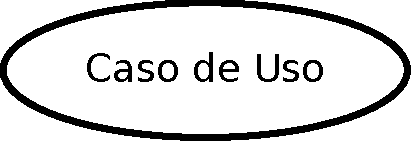
\includegraphics[keepaspectratio,width=.5\textwidth]{Caso_de_Uso}

\begin{alertblock}{Caso de Uso}
Casos de Uso representam o que um dado sistema deve fazer. Entretanto, um caso de uso não representa apenas o que o sistema deve fazer, mas sim o comportamento do sistema quando um dado ator o está utilizando.
\end{alertblock}

\end{frame}

\begin{frame}{Diagrama de Casos de Uso}

\begin{alertblock}{Diagrama de Casos de Uso}
Um diagrama de casos de uso descreve o comportamento do sistema em situações específicas. Logo, o diagrama representa a associação entre atores e casos de uso, assim como (caso existam) são representadas relações entre diferentes casos de uso.
\end{alertblock}

\end{frame}

\begin{frame}{Exemplo de Diagrama de Casos de Uso}

\centering 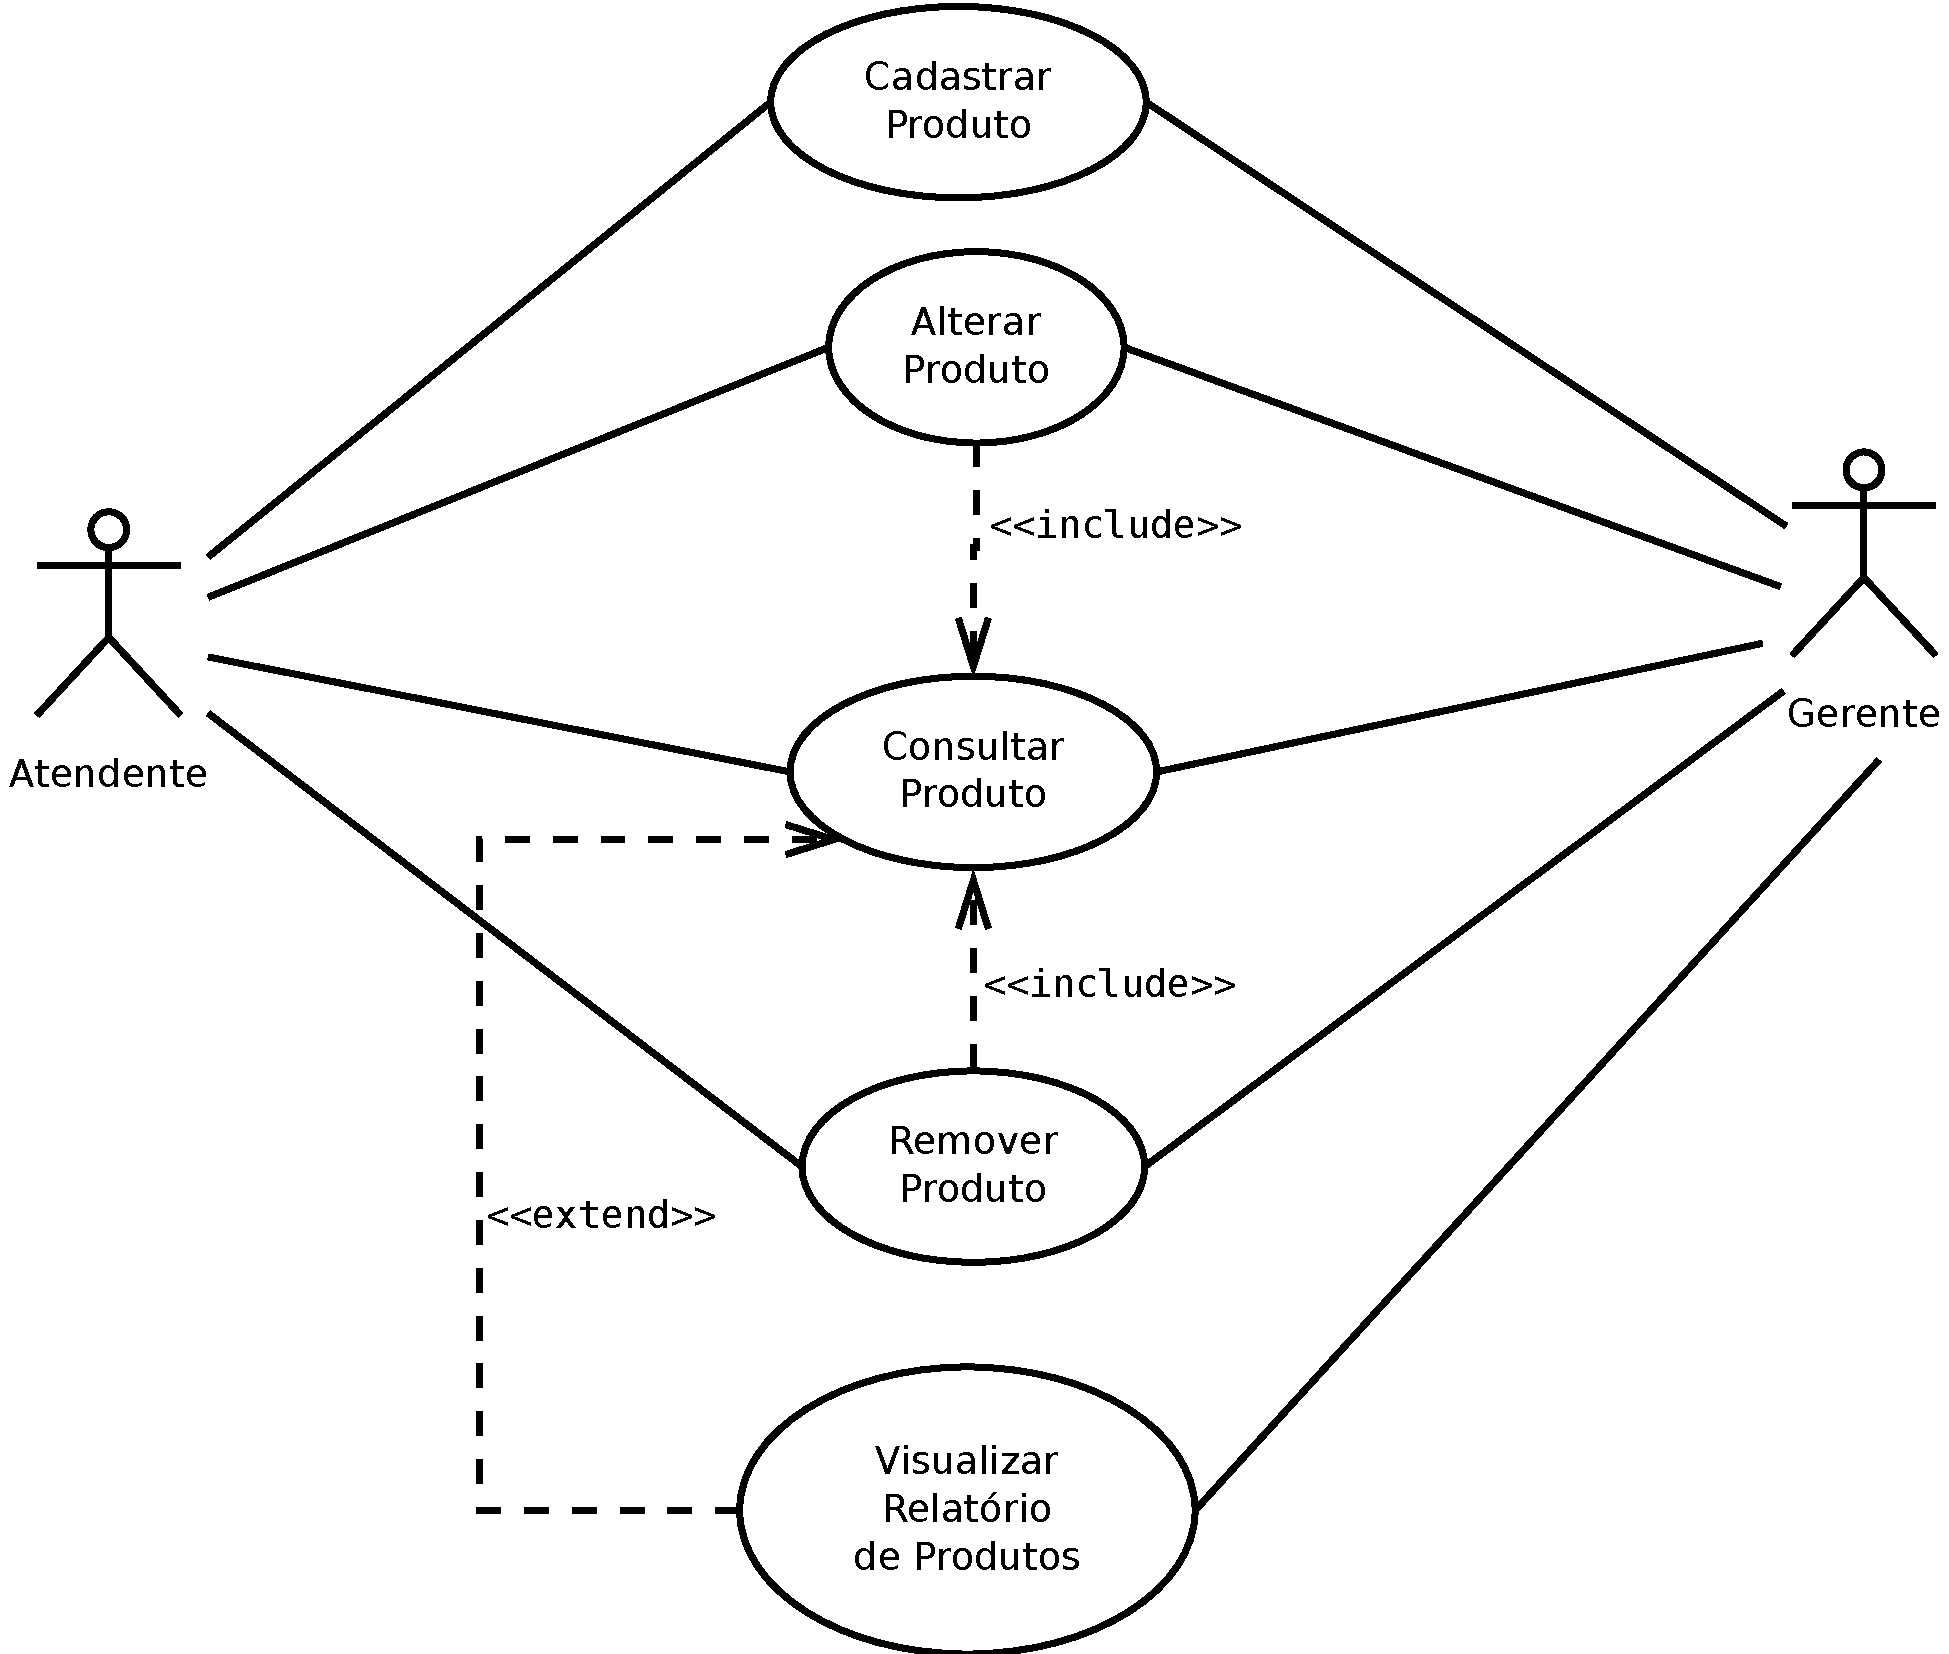
\includegraphics[keepaspectratio,width=.7\textwidth]{Diagrama_Casos_De_Uso_Controle_Estoque}

\end{frame}

\begin{frame}{Exemplo de Descrição de Caso de Uso}

\textbf{Nome}: Cadastrar Produto

\textbf{Descrição}: Este caso de uso permite o cadastro de produtos no sistema de controle de estoques. Diferentes atores (atendente e gerente) podem cadastrar produtos no sistema.\\[5mm]

\textbf{Pré-Condições}: Possuir informações do produto a ser cadastrado.\\[5mm]

\textbf{Pós-Condições}: Caso todas as informações estejam corretas, o novo produto é armazenado na base de dados do sistema. Caso contrário, o produto não é armazenado na base de dados.

\end{frame}

\begin{frame}{Exemplo de Descrição de Caso de Uso}
\textbf{Fluxo normal}:

\begin{enumerate}

\item A qualquer momento antes de salvar o novo produto na base de dados do sistema, o Usuário (Atendente ou Gerente) pode cancelar o cadastro do produto;

\item Usuário (Atendente ou Gerente) seleciona tipo de produto a ser cadastrado;

\item Usuário (Atendente ou Gerente) preenche as informações do produto a ser cadastrado (código, descrição, quantidade, etc..);

\item Usuário (Atendente ou Gerente) salva o produto na base de dados do sistema.

\end{enumerate}
\end{frame}

\begin{frame}{Exemplo de Descrição de Casos de Uso}

\textbf{Fluxos alternativos}:

\vspace*{2mm}

\textbf{Condição 2}: Usuário (Atendente ou Gerente) tenta cadastrar produto já existente na base de dados do sistema.

\begin{enumerate}

\item Ao tentar cadastrar o produto na base de dados do sistema, o Usuário (Atendente ou Gerente) recebe um alerta do sistema indicando que o produto a ser salvo já existe na base de dados;

\item Após emitir o alerta para o Usuário (Atendente ou Gerente) o sistema indica os campos que devem ser únicos, ou seja, não podem pertencer a mais nenhum produto. O Usuário (Atendente ou Gerente) então decide o que fazer;

\item Se o Usuário (Atendente ou Gerente) alterar as informações para cadastrar um novo produto, o produto é salvo na base de dados do sistema. Caso contrário, O Usuário (Atendente ou Gerente) cancela o cadastro.

\end{enumerate}

\end{frame}

\begin{frame}[allowframebreaks]{Exemplo de Descrição de Casos de Uso}

\textbf{Fluxos alternativos}:

\vspace*{5mm}

\textbf{Condição 3}: ...

\textbf{Condição 4}: ...

\textbf{Condição 5}: ...

\begin{alertblock}{\centering \textcolor{red}{Importante!}}
A descrição de um caso de uso não deve ser muito extensa. Portanto, não é preciso especificar uma lista exaustiva de fluxos alternativos. Concentrem-se nos fluxos mais importantes.
\end{alertblock}

\end{frame}

\begin{frame}{Exercício de Fixação}

\begin{alertblock}{Exercício}
Escreva a descrição do caso de uso \textbf{Remover Produto}.
\end{alertblock}

\end{frame}

\begin{frame}{Inclusão de Casos de Uso}

\begin{alertblock}{Inclusão (Include)}
As vezes se faz necessária a utilização de um caso de uso dentro de outro, principalmente quando um determinado comportamento é comum a partes diferentes do sistema. Quando o comportamento de um caso de uso é parte obrigatória de outros casos de uso, utiliza-se a inclusão (<<include>>).

\end{alertblock}

\end{frame}

\begin{frame}{Exemplo de Inclusão de Casos de Uso}

\centering 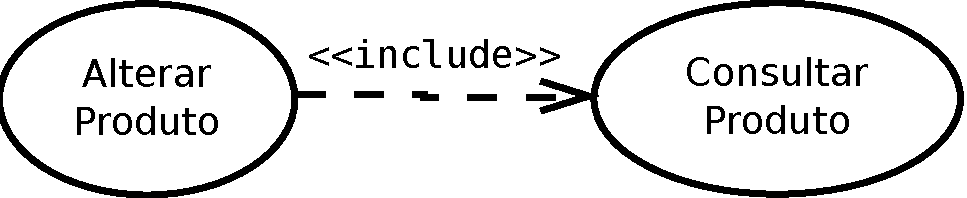
\includegraphics[keepaspectratio,width=.8\textwidth]{Include_Caso_de_Uso}

\begin{alertblock}{Detalhes}
No exemplo acima, o caso de uso \textbf{Consultar Produto} é incluído como parte obrigatória do comportamento do caso de uso \textbf{Alterar Produto}. O motivo é simples: é necessário consultar as informações de um produto antes de poder realizar qualquer alteração. Essa inclusão é realizada através de um ponto de inclusão (inclusion point), que especifica exatamente onde o comportamento do caso de uso incluído deve ser executado.
\end{alertblock}

\end{frame}

\begin{frame}{Extensão de Casos de Uso}

\begin{alertblock}{Extensão (Extends)}
Diferente da inclusão que é obrigatória, a extensão (<<extend>>) de casos de uso permite a inclusão de um caso dentro do outro como parte opcional. 

\end{alertblock}

\end{frame}

\begin{frame}{Exemplo de Extensão de Casos de Uso}

\centering 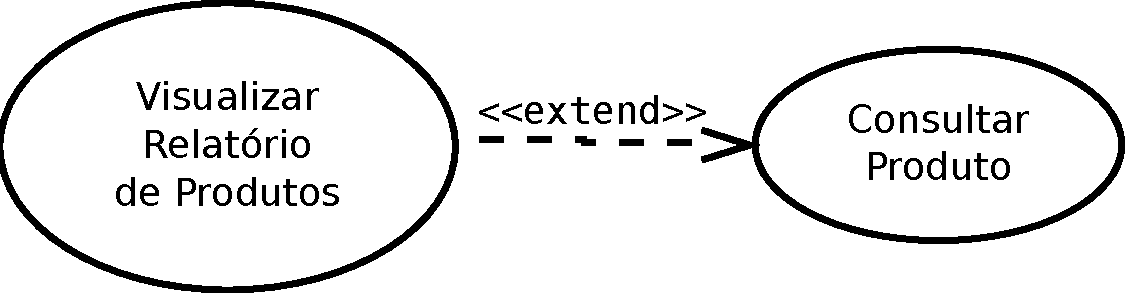
\includegraphics[keepaspectratio,width=.8\textwidth]{Extend_Caso_de_Uso}

\begin{alertblock}{Detalhes}
No exemplo acima, o caso de uso \textbf{Consultar Produto} é incluído como parte opcional do comportamento do caso de uso \textbf{Alterar Produto}. O motivo é simples: a consulta de um deté conerminado produto só é necessária caso o Usuário (Gerente) deseje ver mais detalhes do produto. O uso de extensão de casos de uso é indicado por pontos de extensão (extension points).
\end{alertblock}

\end{frame}

\begin{frame}{Exemplo de Pontos de Extensão}

\centering 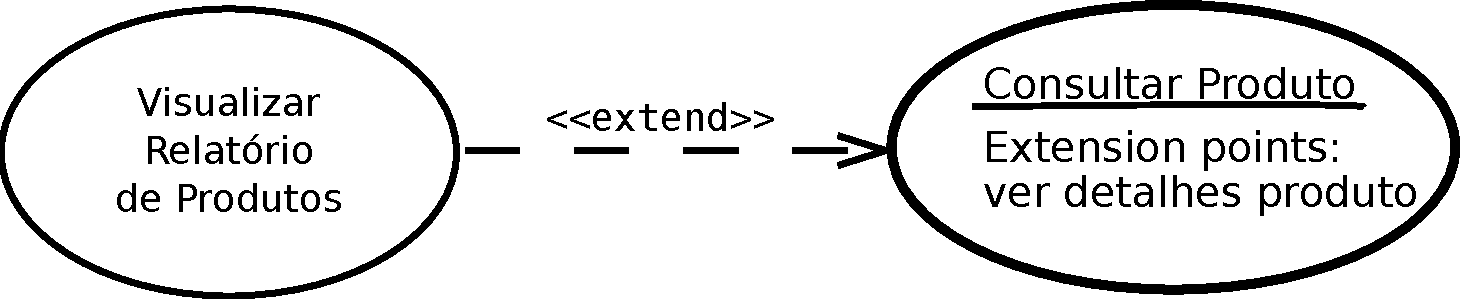
\includegraphics[keepaspectratio,width=.8\textwidth]{Extend_Caso_de_Uso-extension-point}

\begin{alertblock}{Pontos de Extensão (Extension Points)}
Os Pontos de extensão  indicam em que momento e condição a extensão de caso de uso deve ser executada. No exemplo acima, o caso de uso \textbf{Consultar Produto} é executado assim que a condição ver detalhes do produto é disparada. 
\end{alertblock}

\end{frame}

\begin{frame}{Diferenças Entre <<include>> e <<extend>>}

\begin{tabular}{m{7cm}|c|c}
\hline\hline
& \textbf{<<include>>} & \textbf{<<extend>>}\\ 
\hline
O caso de uso é opcional? & Não & Sim
\\ \hline
O caso de uso base completa sem o caso de uso que é incluído/estendido? & Não & Sim \\ 
\hline
A execução do caso de uso é condicionada? & Não & Sim \\
\hline
O caso de uso muda o comportamento do caso de uso base? & Não & Sim \\
\hline\hline
\end{tabular}

\end{frame}

\begin{frame}{Exercício}

\begin{alertblock}{O Desafio da Petshop}
Sua equipe de desenvolvimento foi contratada para desenvolver um sistema para gerir uma petshop. Durrante a fase de levantamento de requisitos, você ficou com a missão de especificar os casos de uso que descrevem o cadastro de clientes, o cadastro de animais associados aos seus clientes, a consulta de informações referentes a um dado animal (ex: ultima vacina realizada, ultima lavagem, última tosagem, etc), e um relatório dos animais que são atendidos pelo estabelecimento. Portanto, especifique um diagrama de casos de uso que complete a sua missão com sucesso :-D. 
\end{alertblock}

\end{frame}

%%%%%%%%%%%%%%%%%%%%%%%%%%%%%%%%%%%%%%%%%%%%%%%%%%%%%%
%%%%%%%%%%%%%%%%%%%%%%%%%%%%%%%%%%%%%%%%%%%%%%%%%%%%%%
\section{}

\begin{frame}[plain,allowframebreaks,noframenumbering]{Bibliografia}

\begin{thebibliography}{Pressman, 2001}

\bibitem[BoochEtAl, 2007]{BoochEtAl-2007}

\newblock{Booch G., Maksimchuk, R. A., Engle, M. W., Young, B. J., Conallen, J., and Houston, K. A. {\em ``Object-Oriented Analysis and Design With Applications"}. 3rd edition. Addison-Wesley, 2007.}

\bibitem[OMG-UML, 2017]{OMG-UML-2017}

\newblock{OMG. {\em ``OMG Unified Modeling Language (OMG UML)"}, version 2.5.1. 2017.}

\bibitem[Pressman, 2001]{Pressman-2001}

\newblock{Pressman, R. {\em ``Software Engineering: A Practioner's Approach"}. 4th edition. McGraw-Hill, 2001.}



\end{thebibliography}

\end{frame}

\begin{frame}[plain,noframenumbering]

\begin{center}

\includegraphics[keepaspectratio, width=.8\textwidth]{template/happycat-end}
\end{center}
\end{frame}

\end{document}